\newprob{1715575628}
{
    下列有關在繩子中傳播的波的敘述,哪項是不正確的?
    \begin{tasks}
        \task 波由振動源產生。
        \task 每個粒子都圍繞各自的平衡位置振動。
        \task 粒子的位移到達最大值時,能量為零。
        \task 能量會在相鄰粒子之間傳遞。
    \end{tasks}

}{
    \mckey C
}

\newprob{1715603438}
{
    一個脈衝以 \qty{1}{cm.s^{-1}} 的速率沿繩子向右傳播。$P$ 是繩子上的一點。在 $t=0$ 時,$P$ 與脈衝相距 1 cm。
    \par{\par\centering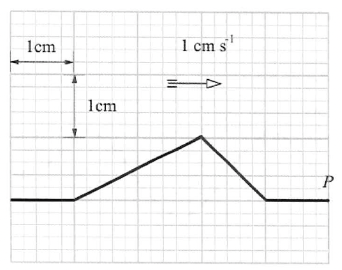
\includegraphics[width=.35\textwidth]{./img/ch1_earlyclass_wave_mc_2024-05-13-20-31-17.png}\par}
    \begin{tasks}(2)
        \task \topalign{\par\centering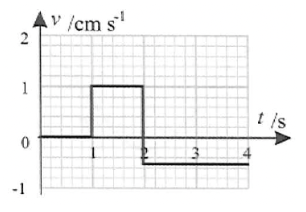
\includegraphics[width=.3\textwidth]{./img/ch1_earlyclass_wave_mc_2024-05-13-20-31-51.png}\par}
        \task \topalign{\par\centering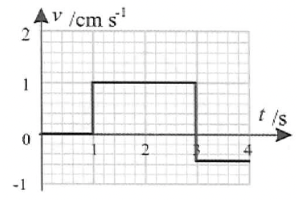
\includegraphics[width=.3\textwidth]{./img/ch1_earlyclass_wave_mc_2024-05-13-20-32-04.png}\par}
        \task \topalign{\par\centering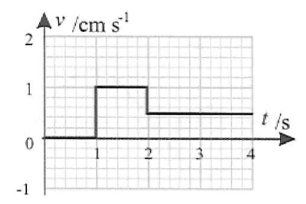
\includegraphics[width=.3\textwidth]{./img/ch1_earlyclass_wave_mc_2024-05-13-20-32-18.png}\par}
        \task \topalign{\par\centering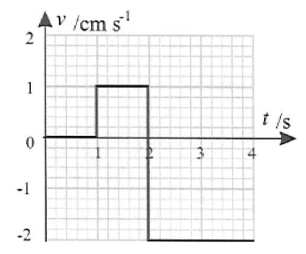
\includegraphics[width=.3\textwidth]{./img/ch1_earlyclass_wave_mc_2024-05-13-20-32-37.png}\par}
    \end{tasks}

}{A}

\newprob{1715587239}
{
    以下顯示一列波在某時刻的位移—距離關係線圖。波的速率是 \vel{0.5}。
    \par{\par\centering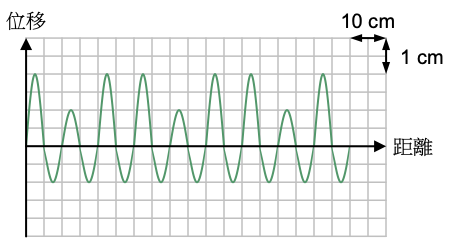
\includegraphics[width=.35\textwidth]{./img/ch1_earlyclass_wave_mc_2024-05-13-16-01-07.png}\par}
    以下哪些敘述是正確的?
    \begin{tasks}
        \task 波的振幅是1.5 cm。
        \task 波的波長是10 cm。
        \task 波的週期是0.6 s。
        \task 以上都不是
    \end{tasks}

}{C}

\newprob{1715587302}
{
    下圖顯示一個拉長了的軟彈簧。
    \par{\par\centering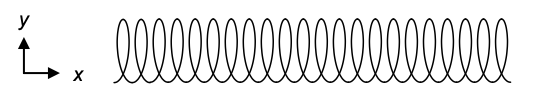
\includegraphics[width=.4\textwidth]{./img/ch1_earlyclass_wave_mc_2024-05-13-16-02-17.png}\par}
    下列哪些敘述是正確的?
    \begin{statements}
        \task 如果一列縱波沿彈簧傳播,彈簧圈會沿方向x振動。
        \task 如果一列橫波沿彈簧傳播,能量會沿方向x傳播。
        \task 一個振動源可同時產生橫波和縱波。
    \end{statements}
    \begin{tasks}
        \task 只有(1)和(2)
        \task 只有(1)和(3)
        \task 只有(2)和(3)
        \task (1), (2) 和 (3)
    \end{tasks}

}{D}

\newprob{1715587436}
{
    一列正弦波以速率1.5 m s–1在一介質內傳播,頻率和振幅分別為2 Hz和
    5 cm。
    \par{\par\centering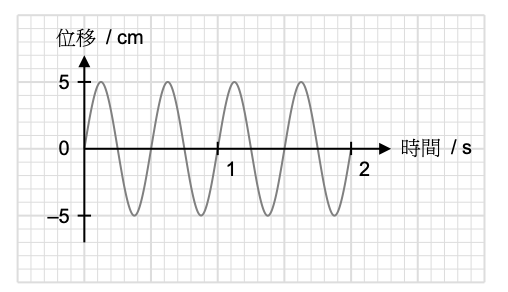
\includegraphics[width=.4\textwidth]{./img/ch1_earlyclass_wave_mc_2024-05-13-16-04-17.png}\par}
    下列哪些是介質中粒子可能的速率?
    \begin{statements}
        \task 0
        \task \vel{0.4}
        \task \vel{1.5}
    \end{statements}
    \begin{tasks}
        \task 只有(1)
        \task 只有(1)和(2)
        \task 只有(2)和(3)
        \task (1), (2) 和 (3)
    \end{tasks}
}{B}

\newprob{1715587507}
{
    下圖顯示一列橫向行波。如果處於A的波峯傳播到B需時3 s,波的速率和頻率是多少?
    \par{\par\centering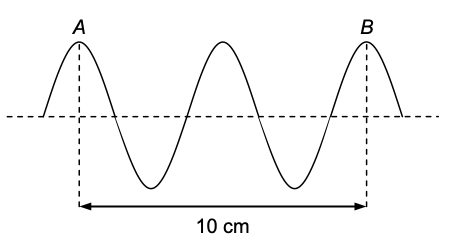
\includegraphics[width=.4\textwidth]{./img/ch1_earlyclass_wave_mc_2024-05-13-16-05-45.png}\par}
    \begin{tasks}
        \task [] \textbf{速率 /m s}$\mathbf{^{-1}}$ \tab\tab \textbf{頻率 /Hz}
        \task 0.0167 \tab\tab 0.333
        \task 0.0167 \tab\tab 0.0167
        \task 0.0333 \tab\tab 0.667
        \task 0.0333 \tab\tab 0.0166
    \end{tasks}

}{C}

\newprob{1715587728}
{
    下圖顯示一列行波 在 $t$ = 0.5 s和$t$ = 1.5 s時的波形。
    \par{\par\centering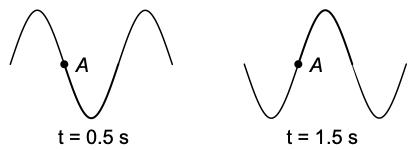
\includegraphics[width=.4\textwidth]{./img/ch1_earlyclass_wave_mc_2024-05-13-16-11-35.png}\par}
    求這個波的最低頻率。
    \begin{tasks}
        \task 0.25Hz
        \task 0.5Hz
        \task 0.75Hz
        \task 1Hz
    \end{tasks}

}{B}

\newprob{1715587962}
{
    一列橫波以 \vel{2} 從$P$傳播到$Q$,下圖顯示粒子$Q$的位移—時間關係線圖。
    \par{\par\centering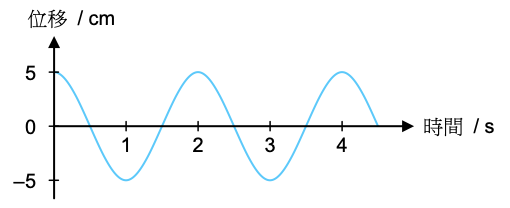
\includegraphics[width=.45\textwidth]{./img/ch1_earlyclass_wave_mc_2024-05-13-16-13-07.png}\par}
    如果$P$和$Q$之間的距離是3 m,下列哪項正確地描述粒子$P$在$t$ = 2 s時的狀態?
    \begin{tasks}
        \task [] \textbf{位移} \tab\tab \textbf{運動}
        \task 0\tab\tab 向上移動
        \task 0\tab\tab 向下移動
        \task 5 cm\tab\tab 靜止
        \task -5 cm \tab\tab 靜止
    \end{tasks}
}{A}

\newprob{1715588106}
{
    下圖顯示一列縱波。
    \par{\par\centering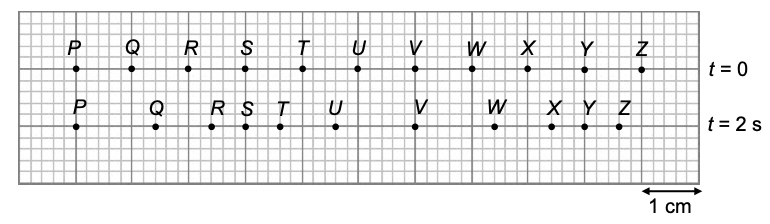
\includegraphics[width=.6\textwidth]{./img/ch1_earlyclass_wave_mc_2024-05-13-16-15-20.png}\par}
    下列哪對粒子的振動反相?
    \begin{tasks}
        \task $P$和$V$
        \task $S$和$Y$
        \task $R$和$T$
        \task $V$和$Y$
    \end{tasks}

}{D}

\newprob{1715588215}
{
    下列哪項有關縱波的敘述是不正確的?
    \begin{tasks}
        \task 所有聲波都是縱波。
        \task 處於密部中心的粒子是瞬間靜止的。
        \task 所有粒子都帶有能量。
        \task 粒子沿波的傳播方向振動。
    \end{tasks}

}{B}

\newprob{1715588251}
{
    以下顯示一列縱波。
    \par{\par\centering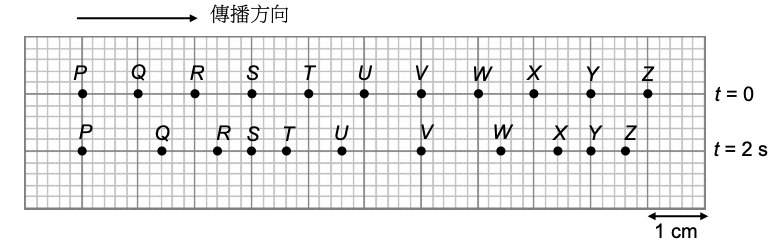
\includegraphics[width=.6\textwidth]{./img/ch1_earlyclass_wave_mc_2024-05-13-16-17-43.png}\par}
    在$t$ = 2 s時,$Q$和$Y$分別往哪個方向運動?
    \begin{tasks}
        \task [] \textbf{Q} \tab\tab \textbf{Y}
        \task 往左 \tab\tab 往左
        \task 往左 \tab\tab 往右
        \task 往右 \tab\tab 往左
        \task 往右 \tab\tab 往右
    \end{tasks}
}{B}

\newprob{1715588357}
{
    如圖所示,一支 659 Hz 的音叉敲擊後發出聲波。已知聲音在空氣中的波長是 \vel{330}。
    \par{\par\centering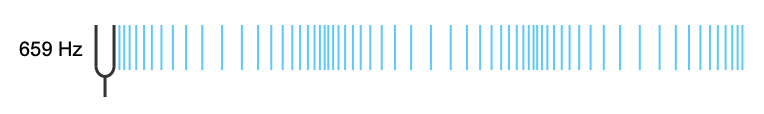
\includegraphics[width=.6\textwidth]{./img/ch1_earlyclass_wave_mc_2024-05-13-16-20-01.png}\par}
    兩個相鄰密部之間的距離是多少?
    \begin{tasks}
        \task 0.25 m
        \task 0.50 m
        \task 0.75 m
        \task 1.00 m
    \end{tasks}

}{B}

\newprob{1715588462}
{
    一列縱波以速率 \vel{3000}在某介質中傳播。以下顯示介質中一個粒子的位移—時間關係線圖,取波的傳播方向為正。
    \par{\par\centering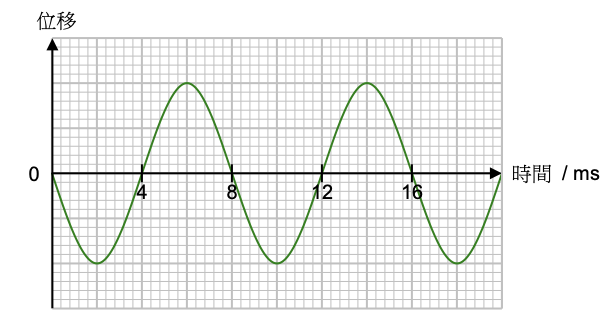
\includegraphics[width=.5\textwidth]{./img/ch1_earlyclass_wave_mc_2024-05-13-16-21-19.png}\par}
    粒子在甚麼時間處於疏部中心?
    \begin{tasks}
        \task $t=4$ \unit{m.s}
        \task $t=6$ \unit{m.s}
        \task $t=8$ \unit{m.s}
        \task $t=10$ \unit{m.s}
    \end{tasks}


}{A}

\newprob{1715588559}
{
    以下顯示一列向右傳播縱波的位移—距離關係線圖,取向右為正。
    \par{\par\centering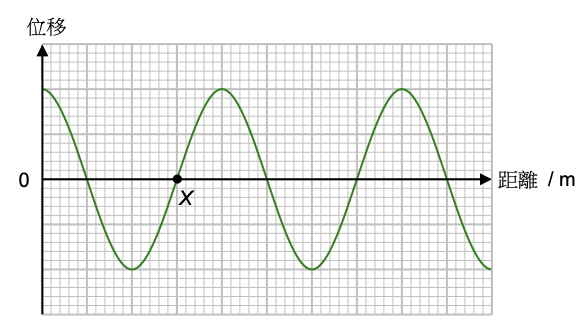
\includegraphics[width=.5\textwidth]{./img/ch1_earlyclass_wave_mc_2024-05-13-16-22-56.png}\par}
    下列哪項有關$X$的敘述是\textbf{不正確}的?
    \begin{tasks}
        \task $X$正處於疏部中心。
        \task $X$正處於平衡位置。
        \task $X$正在向右移動。
        \task $X$正處於最高速率。
    \end{tasks}

}{center}